\begin{apendicesenv}

\chapter{Métricas de Código-Fonte do Apache Maven}
\label{metrics-data}

\begin{table}[ht]
\centering
\begin{tabular}{|l|l|l|l|l|}
\hline
Data da Análise             & Métrica & Média & Mediana & Percentil \\ \hline
\multirow{8}{*}{07/09/2013} & LOC     & 82,7  & 40      & 40        \\ \cline{2-5} 
                            & ACCM    & 2     & 1,3     & 2,7       \\ \cline{2-5} 
                            & ACC     & 2,6   & 1       & 3         \\ \cline{2-5} 
                            & RFC     & 21    & 9       & 23        \\ \cline{2-5} 
                            & LCOM4   & 1,1   & 1       & 1         \\ \cline{2-5} 
                            & NOM     & 7,2   & 4       & 8         \\ \cline{2-5} 
                            & DIT     & 1,2   & 1       & 2         \\ \cline{2-5} 
                            & NOC     & 0,4   & 0       & 1         \\ \hline
\end{tabular}
\label{07/09}
\caption{Métricas de Código Fonte do Apache Maven em 07/09/2013}
\end{table}



\begin{table}[ht]
\centering
\begin{tabular}{|l|l|l|l|l|}
\hline
Data da Análise             & Métrica & Média & Mediana & Percentil \\ \hline
\multirow{8}{*}{13/10/2013} & LOC     & 89,5  & 40      & 40        \\ \cline{2-5} 
                            & ACCM    & 1,8   & 1       & 2         \\ \cline{2-5} 
                            & ACC     & 2,6   & 1       & 3         \\ \cline{2-5} 
                            & RFC     & 20,8  & 8       & 23        \\ \cline{2-5} 
                            & LCOM4   & 1,1   & 1       & 1         \\ \cline{2-5} 
                            & NOM     & 7,2   & 4       & 8         \\ \cline{2-5} 
                            & DIT     & 1,2   & 1       & 2         \\ \cline{2-5} 
                            & NOC     & 0,4   & 0       & 1         \\ \hline
\end{tabular}
\label{13/10}
\caption{Métricas de Código Fonte do Apache Maven em 13/10/2013}
\end{table}



\begin{table}[ht]
\centering
\begin{tabular}{|l|l|l|l|l|}
\hline
Data da Análise             & Métrica & Média & Mediana & Percentil \\ \hline
\multirow{8}{*}{20/10/2013} & LOC     & 89,5  & 40      & 40        \\ \cline{2-5} 
                            & ACCM    & 1,8   & 2       & 2         \\ \cline{2-5} 
                            & ACC     & 2,6   & 1       & 3         \\ \cline{2-5} 
                            & RFC     & 20,8  & 8       & 23        \\ \cline{2-5} 
                            & LCOM4   & 1,1   & 1       & 1         \\ \cline{2-5} 
                            & NOM     & 7,2   & 4       & 8         \\ \cline{2-5} 
                            & DIT     & 1,2   & 1       & 2         \\ \cline{2-5} 
                            & NOC     & 0,4   & 0       & 1         \\ \hline
\end{tabular}
\label{20/10}
\caption{Métricas de Código Fonte do Apache Maven em 20/10/2013}
\end{table}


\begin{table}[ht]
\centering
\begin{tabular}{|l|l|l|l|l|}
\hline
Data da Análise             & Métrica & Média & Mediana & Percentil \\ \hline
\multirow{8}{*}{27/10/2013} & LOC     & 89,5  & 40      & 40        \\ \cline{2-5} 
                            & ACCM    & 1,8   & 2       & 2         \\ \cline{2-5} 
                            & ACC     & 2,6   & 1       & 3         \\ \cline{2-5} 
                            & RFC     & 20,8  & 8       & 23        \\ \cline{2-5} 
                            & LCOM4   & 1,1   & 1       & 1         \\ \cline{2-5} 
                            & NOM     & 7,2   & 4       & 8         \\ \cline{2-5} 
                            & DIT     & 1,2   & 1       & 2         \\ \cline{2-5} 
                            & NOC     & 0,4   & 0       & 1         \\ \hline
\end{tabular}
\label{27/10}
\caption{Métricas de Código Fonte do Apache Maven em 27/10/2013}
\end{table}


\begin{table}[ht]
\centering
\begin{tabular}{|l|l|l|l|l|}
\hline
Data da Análise             & Métrica & Média & Mediana & Percentil \\ \hline
\multirow{8}{*}{03/11/2013} & LOC     & 89,5  & 40      & 40        \\ \cline{2-5} 
                            & ACCM    & 1,8   & 2       & 2         \\ \cline{2-5} 
                            & ACC     & 2,6   & 1       & 3         \\ \cline{2-5} 
                            & RFC     & 20,8  & 8       & 23        \\ \cline{2-5} 
                            & LCOM4   & 1,1   & 1       & 1         \\ \cline{2-5} 
                            & NOM     & 7,2   & 4       & 8         \\ \cline{2-5} 
                            & DIT     & 1,2   & 1       & 2         \\ \cline{2-5} 
                            & NOC     & 0,4   & 0       & 1         \\ \hline
\end{tabular}
\label{03/11}
\caption{Métricas de Código Fonte do Apache Maven em 03/11/2013}
\end{table}


\begin{table}[ht]
\centering
\begin{tabular}{|l|l|l|l|l|}
\hline
Data da Análise             & Métrica & Média & Mediana & Percentil \\ \hline
\multirow{8}{*}{10/11/2013} & LOC     & 89,5  & 40      & 40        \\ \cline{2-5} 
                            & ACCM    & 1,8   & 2       & 2         \\ \cline{2-5} 
                            & ACC     & 2,6   & 1       & 3         \\ \cline{2-5} 
                            & RFC     & 20,8  & 8       & 23        \\ \cline{2-5} 
                            & LCOM4   & 1,1   & 1       & 1         \\ \cline{2-5} 
                            & NOM     & 7,2   & 4       & 8         \\ \cline{2-5} 
                            & DIT     & 1,2   & 1       & 2         \\ \cline{2-5} 
                            & NOC     & 0,4   & 0       & 1         \\ \hline
\end{tabular}
\label{03/11}
\caption{Métricas de Código Fonte do Apache Maven em 10/11/2013}
\end{table}


\chapter{Descrição Simplicada do Processo de ETL no Kettle}

\label{implementação}

No Kettle, o processo de ETL foi modelado de forma a obter a métricas do código-fonte do projeto. Para isso, executa-se um Job, que é o componente de fluxo de controle tal como se mostra na Figura \ref{job}.


\begin{figure}[ht!]
\centering
\includegraphics[keepaspectratio=false,scale=0.60]{figuras/JOB.eps}
\caption{\textit{Job} no Kettle}
\label{job}
\end{figure}
\FloatBarrier

Esse \textit{Job} envolve uma série de transformações para que se alcance o resultado final, que são as métricas de código-fonte agregadas em nível do projeto no \textit{Data Warehouse}.


A primeira \textit{Trasformation} envolve gravar os dados do projeto, que advém de um arquivo JSON extraído do SonarQube no DW, por meio dos componentes do Kettle, tal como se mostra na Figura \ref{first}.


\begin{figure}[ht!]
\centering
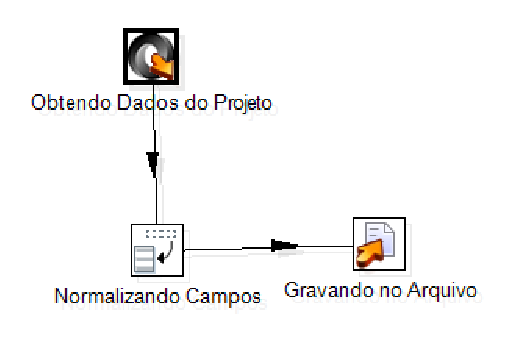
\includegraphics[keepaspectratio=false,scale=0.8]{figuras/first.eps}
\caption{Primeira \textit{Trasformation} do ETL}
\label{first}
\end{figure}
\FloatBarrier



A segunda \textit{Trasformation}, que tem nome de  "Calculando as Métricas", é a principal \textit{Trasformation} do ETL. O fluxo desta é demostrado na Figura \ref{segundatransformation}, 

\begin{figure}[ht!]
\centering
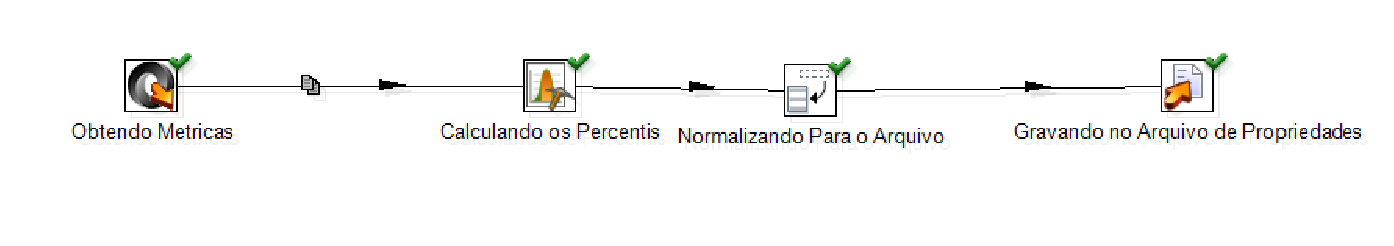
\includegraphics[keepaspectratio=false,scale=0.75]{figuras/fluxoarquivo.eps}
\caption{Segunda \textit{Transformation} do ETL}
\label{segundatransformation}
\end{figure}
\FloatBarrier



O processamento da segunda \textit{Trasformation} inicia-se com a leitura de um arquivo JSON semelhante ao expresso abaixo:

\lstinputlisting[language=Javascript,firstnumber=1,caption=Exemplo de Métricas de uma classe em JSON]{apendices/examplejson.js}


O processamento do JSON é realizado, então, com o componente \textit{JSON input} do Kettle, tal como se mostra a Figura \ref{dadosjson}.



\begin{figure}[ht!]
\centering
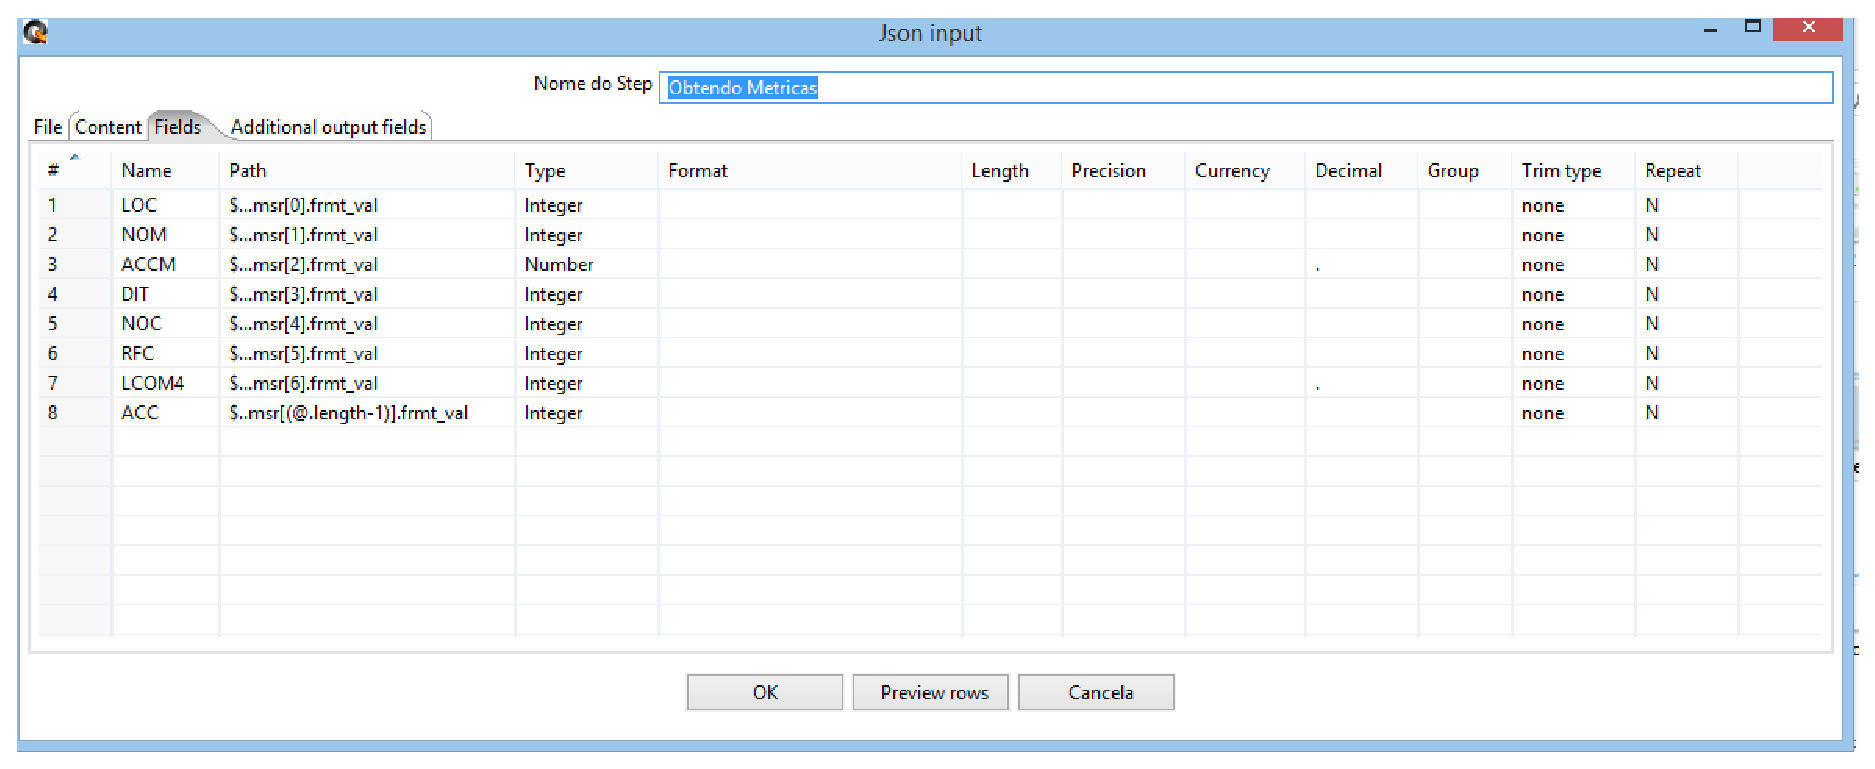
\includegraphics[keepaspectratio=false,scale=0.55]{figuras/dadosjson.eps}
\caption{Obtendo os Dados do JSON}
\label{dadosjson}
\end{figure}
\FloatBarrier

Este resulta na obtenção, no ambiente do Ketle, das métricas de código-fonte que serão agregadas para se obter os valores dos percentis de cada métrica, tal como se vê na Figura \ref{jsonoutput}.


\begin{figure}[ht!]
\centering
\includegraphics[keepaspectratio=false,scale=0.45]{figuras/jsonoutput.eps}
\caption{Resultado do Processamento do \textit{JSON input}}
\label{jsonoutput}
\end{figure}
\FloatBarrier

Após a realização da agregação estatística com os percentis obtém-se um resultado semelhante a Figura \ref{percentils}.


\begin{figure}[ht!]
\centering
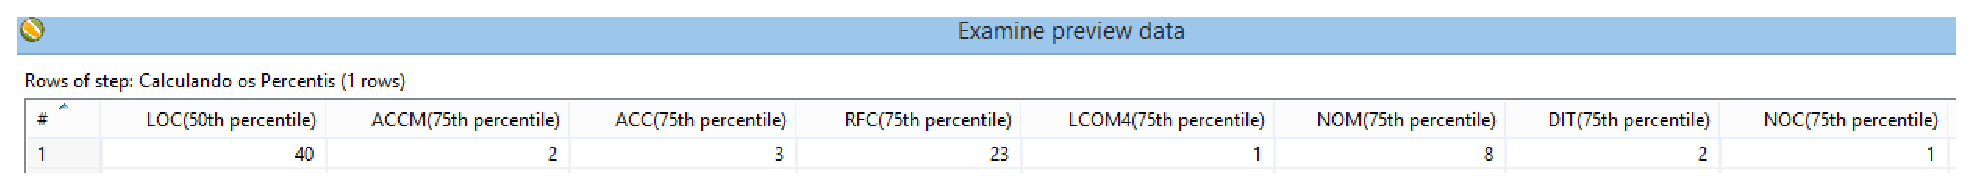
\includegraphics[keepaspectratio=false,scale=0.50]{figuras/percentils.eps}
\caption{Resultado do Processamento Estatístico das Métricas de Código-Fonte}
\label{percentils}
\end{figure}
\FloatBarrier

A terceira \textit{Trasformation} envolve a criação de registro na dimensão Tempo tal como se mostra na Figura \ref{third}.


\begin{figure}[ht!]
\centering
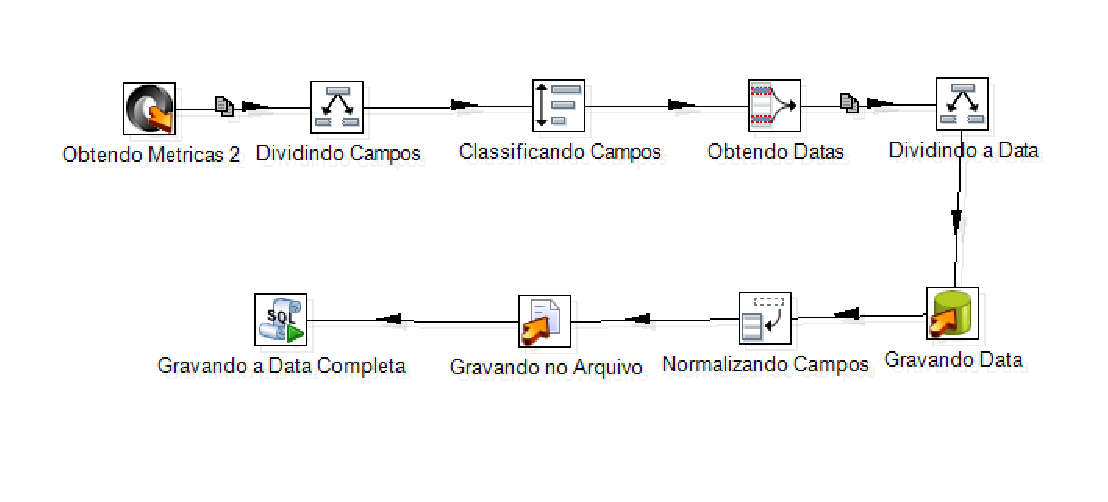
\includegraphics[keepaspectratio=false,scale=0.85]{figuras/third.eps}
\caption{Terceira \textit{Transformation} do ETL}
\label{third}
\end{figure}
\FloatBarrier

Por fim a quarta \textit{Trasformation} realiza a partir do arquivo de propriedades no qual foi gravado todos os registros das dimensões, a carga do fatos do DW tal como se mostra na Figura \ref{fourth}.


\begin{figure}[ht!]
\centering
\includegraphics[keepaspectratio=false,scale=0.80]{figuras/fourth.eps}
\caption{Quarta \textit{Transformation} do ETL}
\label{fourth}
\end{figure}
\FloatBarrier

Todos os arquivos das transformações, jobs e etc podem ser encontrados, com detalhes, no repositório Github: \url{https://github.com/gbrego/TCC}.

\end{apendicesenv}
